\documentclass[../thesis/thesis.tex]{subfiles}
\renewcommand{\baselinestretch}{1.5}\selectfont
\graphicspath{{../figs/ch3-measunc/}}

\begin{document}
	
\onlyinsubfile{\setcounter{chapter}{2}}

%\begin{refsection}
\chapter{Measurement Uncertainty}
\section{Introduction}

A measurement is an observation of a physical effect or quantity which provides useful information. This information, through the ages, has been used to facilitate advancement of both scientific knowledge and industrial development - from the production of standardised stone blocks to build the pyramids of ancient Egypt, to the production of standardised car parts to build Henry Ford's Model T. In the scientific realm, advanced measurement techniques at laboratories such as CERN are used to convince the world that new subatomic particles exist.

To communicate information about a measurement, the recipient needs to be able to either make or imagine a similar observation to that of the original measurer (or metrologist). The simplest way of doing this is to provide the recipient with the same physical effect or quantity for which to make their own observation (if you require a new nut for a bolt from a hardware shop, you might intuitively take the bolt with you), however, this can be inconvenient or impractical with larger objects, or if the recipient is located far away. Instead, you might substitute a more portable representation. For example, if you were to measure the size of a doorway to see if a new piece of furniture may fit through it, you might cut a piece of string to the same length and use this as the representation of the width of the item. However, this approach is very wasteful and also impractical for many physical effects (temperature, flow, pressure).

A solution widely thought to have been first established in the 3rd or 4th Millennium BC (see Figure \ref{ch3_fig_cubit}), is a system of units. In such a system, a discretised value of a quantity is standardised and knowledge of its value is disseminated to all people who wish to use it. Typically, a range of discrete values are chosen, such that the system of units can be conveniently used to represent all measurements. Knowledge of the discretised values is obtained from a primary standard which becomes the definition of the unit and is used to create copies of the standard which can be given to users of the unit system to perform measurements with. The most common method of performing measurements with a unit system is to use a standard to calibrate a measuring instrument, which can then be used to measure an arbitrary value of a quantity in the units defined by the standard.

\begin{figure}
	\centering
	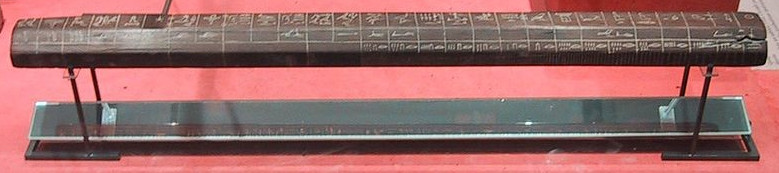
\includegraphics[width=\textwidth]{cubit}
	\caption[Egyptian royal cubit rod of Maya.]{Egyptian royal cubit rod of Maya (treasurer of King Tutankhamun) 1336--1327 BC. The cubit is thought to be the earliest attested standard measure of length, first used in the 3rd or 4th Millennium BC.}
	\label{ch3_fig_cubit}
\end{figure}

The introduction of a regulated system of units enables commerce, as traded goods can be reliably valued between merchants across cities. This application is encountered by all citizens, and so there is a high demand for standards to be produced from the primary standard and physically distributed. It becomes impractical to create all standards by copying the primary standard directly (in some cases because the value of the primary standard is perturbed each time it is measured), and so a tiered organisational structure of standards is used. In this structure, there is a tier consisting of a small number of standards which are created directly from measurements of the primary standard, followed by subsequent tiers of larger numbers of standards which are derived from measurements of those in the previous tier. For any standard produced, it should be possible to trace the lineage back to a measurement of the primary standard. This is referred to as a traceability chain (see Figure \ref{ch3_fig_traceability}) and it is a fundamental tenet of metrology. Measurements with a shorter traceability chain are considered more traceable than those with longer chains.

\begin{figure}
	\centering
	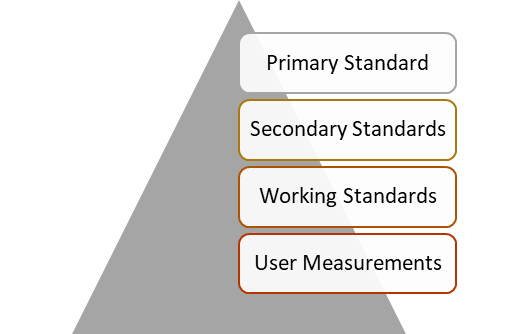
\includegraphics[]{traceability}
	\caption[An illustration of measurement traceability.]{The traceability chain, where the pyramid shows the number of instances of standards in each tier. Secondary standards are held at NMIs and used to periodically calibrate working standards, which are sent by manufacturers and laboratories. User measurements are made using instruments calibrated with these working standards, so they number the greatest and are at the bottom of the traceability chain.}
	\label{ch3_fig_traceability}
\end{figure}

Today, the primary standards are maintained in most countries by a National Measurement Institute (NMI) and co-ordinated by the Bureau of International Weights and Measures (BIPM). To accommodate international trade and compatibility, a routine process of inter-comparisons is undertaken to ensure that the values of the primary standards between countries are in agreement.

Secondary standards are also kept by the NMIs and are used to reduce excessive wear to the primary standard caused by frequent measurements (and also to reduce bottlenecks caused by having a single standard). They are calibrated against the primary standard as infrequently as possible, again to reduce wear. Secondary standards are used by the NMI to characterise working standards which are sent to them by manufacturers and research institutes. Another important task of each NMI is to perform investigations to discover new and improved methods of measurement, which make use of secondary standards to better compare the accuracy of different methods.

Working standards are used, for example, by instrumentation manufacturers who may use them to calibrate their products before shipping to the customer, and more generally the standards can be used to calibrate test equipment to identify faulty products. Larger research institutes typically use working standards to recalibrate instrumentation prior to performing very sensitive measurements. To ensure that product specifications and scientific measurements are traceable and of high quality, accreditation services such as the United Kingdom Accreditation Service (UKAS) exist to certify manufacturers and laboratories that demonstrate good measurement practice and use traceable measurements \cite{UKAS}.

The selection of quantities for which primary standards are kept is only a subset of those for which recognised units exist. This is because many units are derived quantities, where their value can be obtained by calculation using definitions of other units. For example, the definition of the unit of resistance ($R$, ohms) can be derived from that of voltage ($V$, volts) and current ($I$, amperes), because $R=V/I$. The eight fundamental ``base'' units which make up the International System of Units (SI), are the metre, kilogram, second, ampere, kelvin, candela and mole. From these unit definitions, it is possible to define any other derived unit in use. NMIs will usually keep secondary standards of most derived quantities that users may wish to calibrate against, which are traceable to one or more primary standards of the base units. Although traditionally all primary standards were defined by physical artefacts (e.g. metallic weights, burning candles), these are being gradually replaced by definitions involving physical constants (e.g. Plank, Boltzmann), which do not degrade over time or use. The ``Ninth SI Units'' \cite{SI}, a proposition recently accepted by the BIPM, covers the redefinition of four of the SI units (the ampere, the kilogram, the kelvin and the mole) which is scheduled for May 2019.

The crucial effect of traceability on measurements is the confidence in their results. Measurements with poor traceability (longer chains) will produce results which are likely to be less accurate than those with better traceability (shorter chains). The reason for this is measurement uncertainty, which will now be explained.

It is impossible to know the true value of a quantity being measured as many undesirable physical effects typically occur during the measurement process. These effects contribute error (an unwanted perturbation) to the measured value, causing a reduction in accuracy (the deviation of the  measured value from the true value). Typical sources of error in measurement include thermal noise, imperfect calibration and drift of environmental conditions from those at which a measuring instrument was calibrated. In some cases, it is possible to quantify and correct for these errors, but there are often many sources (some of which contribute very small errors) which cannot be corrected for. This is because either the error cannot be quantified or the value of the error will change over the duration of the measurement process (random errors). Any source of error which cannot be removed from a measurement becomes a source of uncertainty, because the deviation of the measured value from the true value due to this source of error is uncertain. If it is possible to quantify the amount of uncertainty in a measurement, then a degree of confidence can be formed about its value.
If every measurement has an associated uncertainty in its value, then any measurement involving the results of previous measurements will include uncertainty contributions from both measurements. Measurements with good traceability involve fewer sources of uncertainty than those with poor traceability, leading to a higher degree of confidence in the former. It is because of this fact that NMIs strive to reduce the uncertainties in their primary standard definitions, which in turn reduces the uncertainty in all traceable measurements.

Because it is impossible to know the amount of error in a source of uncertainty, probability and statistical theories are used to instead describe the amount of uncertainty associated with it. By the nature of these theories there are often several methods which can be used to obtain a result, which sometimes provide different values. To ensure consistency and portability of uncertainty definitions, measurement guides were created in each industry and area of science, which specialised in processing the results of typical measurements. In addition, different guides were produced depending on the level of accuracy required - as more accurate measurements often require more effort to complete. Although this practice allowed suitable measurement comparisons within each field (e.g. chemistry, mechanical engineering), ambiguities still existed in uncertainty definitions between fields. To address this, a landmark document was published in 1993 by the International Organisation for Standardisation (ISO), the Guide to the Expression of Uncertainty in Measurement (GUM) \cite{GUM_1993}. This document was the work of representatives from seven international organisations: the BIPM, the International Organisation of Legal Metrology (OIML), the International Electrotechnical Commission (IEC), the ISO, the International Federation of Clinical Chemistry and Laboratory Medicine (IFCC), the International Union of Pure and Applied Chemistry (IUPAC), and the International Union of Pure and Applied Physics (IUPAP). The GUM, updated in 2008 \cite{GUM_2008}, is still used today as a reference for the evaluation of measurement uncertainty in many laboratories and industries across the world. The seven original organisations which wrote the GUM, together with the International Laboratory Accreditation Cooperation (ILAC, of which UKAS is a member), form the Joint Committee for Guides in Metrology (JCGM), who maintain the GUM and subsequent additional documents. These additional documents consist of the International Vocabulary of Metrology (VIM) \cite{VIM} and two supplements to the GUM \cite{GUM_S1,GUM_S2}: Supplement 1 covers the use of a Monte Carlo method \cite{Metropolis_1949} in uncertainty evaluation; Supplement 2 is used where more than one quantity is measured at the same time (multivariate).

Throughout this dissertation, the methodologies presented in the GUM will be used. The international authority of the guide, developed by seven international organisations (including the two global standardisation bodies IEC and ISO), gives strong motivation to use it as a basis for a framework to evaluate uncertainty in measurement.

This Chapter describes the evaluation of uncertainty prescribed in the GUM and highlights an inconsistency in the current version of the GUM and associated documents (which can have a profound effect on electromagnetic measurements).

\section{The Measurement Process}

In contrast to basic evaluations of uncertainty, where only repeat measurements of the quantity of interest are analysed, the GUM prescribes a more rigorous approach, which defines a mathematical model of the measurement process (measurement model) and propagates uncertainty through that model to the result (measurands). This allows any uncertainties from previous measurements, including those involving standards in the traceability chain, to be included in the result. The measurement model can be simple, such as measuring resistance using input quantities of voltage and current, or complicated and multivariate, requiring many input quantities and producing many output quantities. In some cases, the measurement model may not be known and can be defined as a black box, but this has certain limitations discussed later with Monte Carlo methods.

The GUM defines a process that is to be followed when evaluating uncertainty in measurement. It consists of the following steps:

\begin{enumerate}
	\item Modelling the measurement.
	\item Evaluating standard uncertainty of input quantities.
	\item Determining combined standard uncertainty of the measurands.
	\item Determining expanded uncertainty of the measurands.
\end{enumerate}

where standard uncertainty is an uncertainty expressed as a standard deviation and expanded uncertainty is used to define a coverage interval encompassing a large fraction of the distribution of values that could reasonably be attributed to the measurand.

\subsection{Modelling the Measurement}

The VIM document \cite{VIM} defines a measurement model\footnote{The definition of model used in ``measurement model'' is different to that used when describing models of amplifiers seen elsewhere in this dissertation.} as ``a mathematical relation among all  quantities known to be involved in a measurement''. In many cases, where an explicit relation can be written, it is possible to further define a measurement function. We can represent this generally as a set of measurands $Y$ having a functional relationship, $f(.)$, depending on $N$ input quantities $X_1, X_2, \dots, X_N$:

\begin{equation}
Y=f(X_1,X_2,\dots,X_N)
\end{equation}

The estimates of the measurands $\bar{Y}$ can be found by evaluating the measurement model using the estimates of each input quantity $\bar{x}_1,\bar{x}_2,\dots,\bar{x}_N$:

\begin{equation}
\bar{Y}=f(\bar{x}_1,\bar{x}_2,\dots,\bar{x}_N)
\end{equation}

Each input quantity could either be observed during the present measurement, a result from a previous measurement, or another source of information such as a datasheet or specification. An example of a measurement model could be for a temperature measurement, where the input quantities would include the value observed from the meter, the previously measured values of two calibration temperatures, and the assumed values of those calibration temperatures. Using this method, uncertainty from the calibration can be included in the evaluation. This is especially true for uncertainties caused by systematic errors, which do not vary during the measurement process and cannot be evaluated purely by performing repeat measurements.

\subsection{Evaluating Standard Uncertainty of Input Quantities}

Sources, or components, of uncertainty in measurement can be divided into two categories: Category A uncertainty components are those that are evaluated using statistical analysis of a series of observations (i.e. repeats); Category B components are those that are evaluated using other means, for example using information from datasheets.

The GUM presents methods that include the use of both Bayesian and classical probabilistic methods to evaluate the uncertainty in the input quantities for a measurement model. In particular, classical methods \cite{Neyman_1937} are used for the treatment of Category A uncertainty components and Bayesian methods \cite{Gelman_2013} are used for the treatment of Category B uncertainty components. This is a sensible assignment as classical (frequentist) methods work well for repeat observations and Bayesian inference can be used to incorporate alternative sources of knowledge. An informative discussion on these types of method can be found in \cite{White_2016}. Since the publication of the GUM, some authors have stated (for example, in \cite{Kacker_2006,Kacker_2005,Kacker_2003,Bich_2014}) that this combination of different probabilistic methods (i.e., Bayesian and classical) represents an inconsistency in the GUM methodology for evaluating measurement uncertainty. The author has published a paper considering the effects of this inconsistency on electromagnetic wave measurements at radio frequencies \cite{Stant_2016}, which forms the basis for this section of the chapter.

The supplements to the GUM \cite{GUM_S1,GUM_S2} resolve the above-mentioned inconsistency by introducing a method for treating the Category A uncertainties that follows a Bayesian approach \cite{Elster_2007}. Therefore, the two supplements no longer contain the inconsistency found in the original GUM document. However, as a consequence of this change, there is now inconsistency between the method used to evaluate uncertainty described in the GUM and that described in the two supplements. In many situations, these different methods do not have a significant impact on the overall uncertainty that is evaluated. For situations where a considerable number of input quantities are observed simultaneously, the two different approaches can produce significantly different values of uncertainty. Such situations often occur in the area of high-frequency electromagnetic metrology, which is the topic of this dissertation.

\subsubsection{Category A Evaluation}

\paragraph{GUM Method}

The classical statistical technique \cite{Neyman_1937} applied to Category A uncertainties in the current GUM is based on a series of observations of a randomly varying input quantity. After $n$ observations $x_1,x_2,\dots,x_n$, the best available estimate (arithmetic mean of measured values), $\bar{x}$, and standard deviation, $s$, of a randomly varying input quantity, $X$, is written as

\begin{align}
\bar{x} & =\frac{1}{n}\sum_{i=1}^{n}x_i,\\
s & =\sqrt{\frac{1}{n-1}\sum_{i=1}^{n}(x_i-\bar{x})^2}
\end{align}

respectively, where $x_i$ is the result of the $i$th observation. Importantly, a minimum of two observations must be made ($n=2$) in order for $\bar{x}$ and $s$ to be defined. The standard uncertainty of the best estimate of $X$, $u(\bar{x})_{\textrm{GUM}}$ can be found by dividing $s$ by the square root of the number of observations:

\begin{equation}
u(\bar{x})_{\textrm{GUM}}=\frac{s}{\sqrt{n}}
\label{ch3_eqn_ux_gum}
\end{equation}

If there are correlated (mutually dependent) input quantities present in the measurement model, the covariances of each pair of input quantities must also be calculated before the propagation of uncertainty. Both the standard uncertainties and the covariances for $N$ input quantities can be represented in a symmetric ($N\times N$) matrix containing the variance of each quantity ($s^2$) along the diagonal and the covariance between $x_i$ and $x_j$ in the $i$, $j$th element. This is called the “uncertainty matrix” in the GUM and the “measurement covariance matrix” in the GUM Supplement 2. An example given in the GUM and described later in this Chapter, demonstrates this scenario using the example of a simultaneous measurement of resistance and reactance with voltage, current and phase as correlated input quantities \cite[Example~H.2]{GUM_2008}. 

Once the uncertainties of the input quantities have been evaluated, they are propagated through the measurement model, as illustrated in Figure \ref{ch3_fig_model}. This requires the sensitivities of the measurand to each input quantity to be calculated to at least a first order approximation (i.e. the partial derivatives of the measurement model known). The estimates of the input quantities are used in the measurement model to obtain the estimate of the measurand. The variances and covariances of the input quantities are combined with the sensitivity coefficients in order to obtain the variance of the measurand. The combined standard uncertainty of the measurand is equal to the positive square root of this value. The result of the measurement process is then presented as the measurand estimate and combined standard uncertainty. Alternatively, the combined standard uncertainty can multiplied by a positive factor to form an expanded measurement uncertainty. From this value, a coverage interval can be derived which states a particular probability that the true value of the measurand is within that range. A more detailed description of propagating uncertainties through the measurement model and presenting the results will be given later in this Chapter, but a brief introduction was given here to help the reader understand research on input quantity uncertainties presented in the remainder of this section.

\begin{figure}
	\centering
	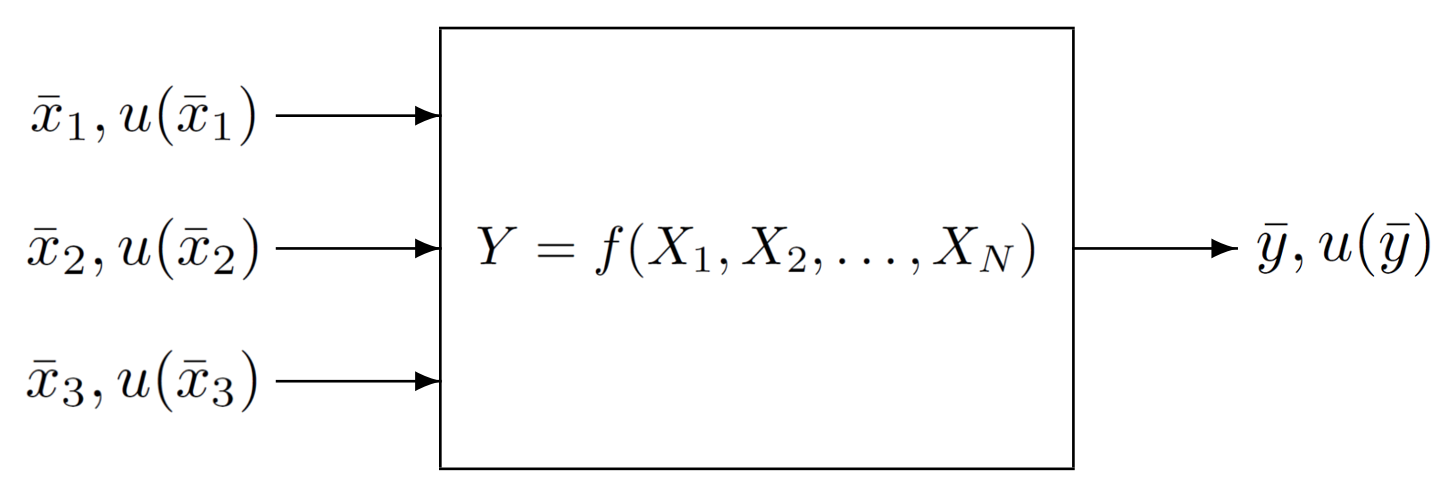
\includegraphics[width=0.65\textwidth]{model}
	\caption[Propagation of measurement uncertainty.]{The propagation of measurement uncertainty through the measurement model, as specified in the GUM. Here, a single measurand $Y$ is shown, but the model could include multiple measurands.}
	\label{ch3_fig_model}
\end{figure}

\paragraph{GUM Supplement Method}

Both GUM supplements (GUM-S1/S2) \cite{GUM_S1,GUM_S2} use a Bayesian approach \cite{Klauenberg_2012} to assign a probability density function (PDF) to all input quantities. This approach results in the choice of a $t$-distribution to characterize Category A input quantities, in contrast to the Gaussian distribution used in the GUM \cite[para. 5.3.2.1]{GUM_S2}. Of particular relevance is the inclusion of the degrees-of-freedom parameter, $\nu$, in the definition of the standard uncertainty and covariances of a $t$-distribution. Whereas for the Gaussian distribution $\nu$ is used as a measure of reliability of the standard uncertainty, it is explicitly required when using the $t$-distribution in order to obtain the standard uncertainty, $u(\bar{x})_{\textrm{SUPP}}$:

\begin{equation}
u(\bar{x})_{\textrm{SUPP}} = \frac{s}{\sqrt{n}} \times \sqrt{\frac{\nu}{\nu-2}},
\label{ch3_eqn_ux_supp_multiv}
\end{equation}

where $\nu=n-N$, with $n$ being the number of observations and $N$ being the number of input quantities. In the GUM-S1 only a univariate $t$-distribution is offered, which represents $N=1$ input quantities. For this case (\ref{ch3_eqn_ux_supp_multiv}) can be rewritten as:

\begin{equation}
u(\bar{x})_{\textrm{SUPP}} = \frac{s}{\sqrt{n}} \times \sqrt{\frac{n-1}{n-3}}.
\label{ch3_eqn_ux_supp_univ}
\end{equation}

Equation \ref{ch3_eqn_ux_supp_univ} is undefined if $n$ is less than four, in which case the standard uncertainty cannot be calculated for a single input quantity according to the guidance given in the GUM-S1 (and the GUM-S2). Figure \ref{ch3_fig_scaling_factor} illustrates the ratio between the standard uncertainty values calculated for different numbers of observations of a single Category A input quantity using the GUM and the GUM-S1/S2 approaches. It can be seen that when $n = 4$, $u(\bar{x})_{\textrm{SUPP}} = \sqrt{3} \times u(\bar{x})_{\textrm{GUM}}$, and as the number of observations increases the results from both approaches converge: If $n$ tends to infinity, the $t$-distribution tends towards a Gaussian distribution. However, most commercial laboratories would avoid making large numbers of measurements as this is often time-consuming and therefore expensive.

\begin{figure}
	\centering
	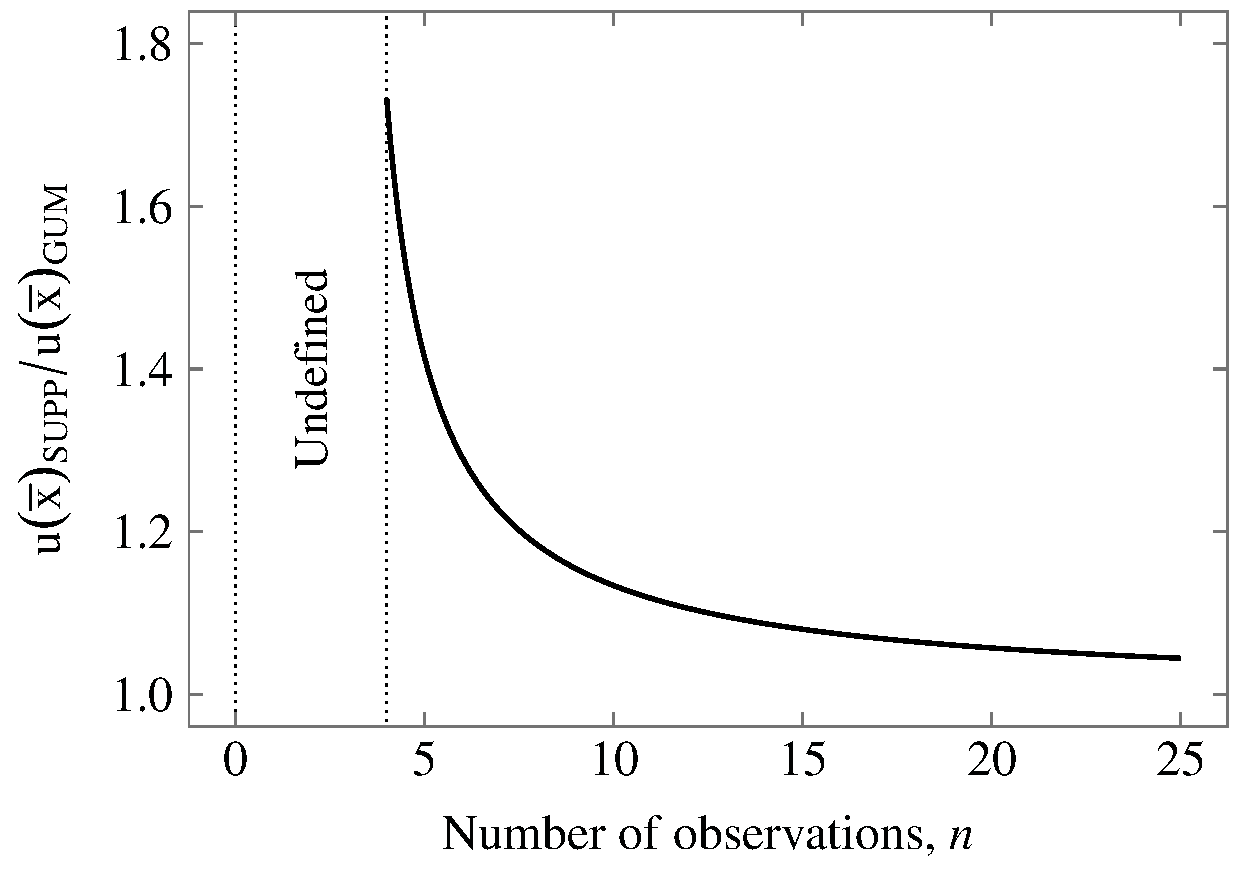
\includegraphics[width=0.65\textwidth]{scaling_factor.pdf}
	\caption{Scaling factor to convert from a GUM standard uncertainty to a GUM Supplement.}
	\label{ch3_fig_scaling_factor}
\end{figure}

For measurements involving multiple input quantities, such as the measurement of a vector quantity, a multivariate/joint distribution should be used as suggested in the GUM-S2. The variances and covariances between all pairs of input quantities are obtained using a matrix form of (\ref{ch3_eqn_ux_supp_multiv}) (\cite[Section~5.3.2]{GUM_S2}):

\begin{align}
\boldsymbol V(\boldsymbol X) & = \frac\nu{(\nu-2)}\frac{\boldsymbol S(\boldsymbol X)}n=\frac1{n(n-N-2)}\sum_{i=1}^n({\boldsymbol x}_i-\overline{\boldsymbol x}){({\boldsymbol x}_i-\overline{\boldsymbol x})}^\top
\\
\boldsymbol S(\boldsymbol X) & = \frac1\nu\hspace{0.35em}\sum_{i=1}^n({\boldsymbol x}_i-\overline{\boldsymbol x}){({\boldsymbol x}_i-\overline{\boldsymbol x})}^\top
\\
\boldsymbol V(\boldsymbol X) & = 
\begin{bmatrix}
u{({\boldsymbol x}_1)}^2&u({\boldsymbol x}_1\text{,}{\boldsymbol x}_2)&\dots&u({\boldsymbol x}_1\text{,}{\boldsymbol x}_n)\\
u({\boldsymbol x}_2\text{,}{\boldsymbol x}_1)&u{({\boldsymbol x}_2)}^2&\dots&u({\boldsymbol x}_2\text{,}{\boldsymbol x}_n)\\
\vdots&\vdots&\ddots&\vdots\\
u({\boldsymbol x}_n\text{,}{\boldsymbol x}_1)&u({\boldsymbol x}_n\text{,}{\boldsymbol x}_2)&\dots&u{({\boldsymbol x}_n)}^2
\end{bmatrix}
\end{align}

where $\bm{U_X}$ is the uncertainty matrix, $\bm{x}_i$ is a sample from the array of vectors containing input quantity indications and $\bar{\bm{x}}$ is the arithmetic mean of that array. For this multivariate case, the minimum value of $n$ will increase linearly with $N$, such that the standard uncertainty is undefined unless $n > N + 2$.

\paragraph{Comparison of GUM and GUM Supplements approach using example H.2/9.4}

Both the GUM and the GUM-S2 provide an identical example which can be used to compare the different standard uncertainties. The example is a simultaneous measurement of resistance and reactance, which uses a measurement model with multiple input quantities and multiple output quantities (measurands). The input quantities are voltage $V$, current, $I$, and phase, $\phi$, and the measurands are resistance $R$, reactance, $X$, and impedance, $Z$. The measurement model is defined as:

\begin{equation}
R=\frac VI\cos\theta, \quad X=\frac VI\sin\theta, \quad Z=\frac VI
\end{equation}

Six sets of observations \cite{VIM} ($n = 6$) of $V$; $I$; $\phi$ are obtained independently by measurement. The version of this example given in the GUM uses only $n = 5$ sets, but one additional set of values of $V$; $I$; $\phi$ has been added for the GUM-S2 example to allow (\ref{ch3_eqn_ux_supp_multiv}) to be defined for $N = 3$ input quantities, a condition which was explained at the end of the previous section. These values, together with their arithmetic means and standard uncertainties as calculated from the two approaches using (\ref{ch3_eqn_ux_gum}) and the matrix form of (\ref{ch3_eqn_ux_supp_multiv}) (which is applicable to measurements involving multiple input quantities), are presented in Table \ref{ch3_tbl_gum_example}. The ratios of the standard uncertainties from each approach is also included in the table, which are identical for all these input quantities due to their dependence only on $n$ and $N$, which are also equal for all these input quantities (e.g. when $n = 6$ and $N = 3$, $\sqrt{(\nu/(\nu-2))}=\sqrt{((n-N)/(n-N-2))}=\sqrt{3}$. This explains why standard uncertainties evaluated with Category A methods using the minimum number of observations following the GUM-S1/S2 approach are always 1.732 times larger than the standard uncertainties calculated following the GUM approach.

\begin{table}[]
	\begin{tabular}{llll} \toprule
		Value             & $V$/V  & $I$/A   & $\phi$/rad   \\ \midrule
		$x_1$             & 5.007  & 19.663  & 1.0456  \\
		$x_2$             & 4.994  & 19.639  & 1.0438  \\
		$x_3$             & 5.005  & 19.640  & 1.0468  \\
		$x_4$             & 4.990  & 19.685  & 1.0428  \\
		$x_5$             & 4.999  & 19.678  & 1.0433  \\
		$x_6$             & 4.999  & 19.661  & 1.0445  \\ \midrule
		$\bar{x}$         & 4.9990 & 19.6610 & 1.04446 \\ \midrule
		$u(\bar{x})\textrm{GUM}$   & 0.0026 & 0.0077  & 0.00061 \\
		$u(\bar{x})\textrm{SUPP}$  & 0.0045 & 0.0134  & 0.0011  \\ \midrule
		$\frac {u(\bar{x})\textrm{GUM}}{u(\bar{x})\textrm{SUPP}}$ & 1.732  & 1.732   & 1.732 \\ \bottomrule
	\end{tabular}
\caption[GUM and GUM Supplement example values.]{The indication values from the example ``Simultaneous Resistance and Reactance Measurement'' and their statistical properties as evaluated by the approaches given in \cite[Example H.2]{GUM_2008} and \cite[Example 9.4]{GUM_S2}.}
\label{ch3_tbl_gum_example}
\end{table}

This difference in the input quantity uncertainties calculated from the two approaches propagates through the measurement model and therefore significantly affects the combined standard uncertainties of the measurands. Table 3.2 presents the combined standard uncertainties of the measurands for the described example as evaluated by both approaches, together with a ratio of the uncertainty values. For all three measurands the combined standard uncertainty calculated using the GUM-S1/S2 method is more than double the equivalent values calculated using the GUM method. For other measurement models with higher sensitivities to the input quantities, this difference could be even greater.

\begin{table}[]
	\begin{tabular}{llll} \toprule
		Method             & $u(R)$/$\Omega$  & $u(X)$/$\Omega$   & $u(Z)$/$\Omega$   \\ \midrule
		GUM                & 0.058 & 0.241 & 0.193 \\
		GUM-S2             & 0.130 & 0.540 & 0.431 \\ \midrule
		$\frac {\textrm{GUM-S2}}{\textrm{GUM}}$ & 2.241  & 2.241   & 2.233 \\ \bottomrule
	\end{tabular}
	\caption[GUM and GUM supplement example results comparison.]{A comparison of the results obtained for the example ``Simultaneous Resistance and Reactance Measurement'' using the approaches given in \cite[Example H.2]{GUM_2008} and \cite[Example 9.4]{GUM_S2}.}
	\label{ch3_tbl_gum_compare}
\end{table}

\paragraph{Comparison of GUM and GUM Supplements approach using microwave scattering parameters example}

High-frequency electromagnetic metrology often involves using multiple complex-valued quantities. Common input quantities for this type of measurement, measured using instruments such as vector network analysers (VNA), are scattering parameters (S-parameters), as described in Chapter 2. Because each S-parameter is a complex-valued quantity ($S = (S_{\textrm{Re}}, S_{\textrm{Im}})$), there are $2m^2$ input quantities required in a measurement model for the complete response of an $m$ port device. All these quantities are correlated, so a multivariate distribution should be used to represent them. It has been shown previously that for a Category A evaluation of uncertainty, both the number of repeat observations and the number of input quantities have a significant effect on the difference in uncertainty as calculated from the two approaches presented in the GUM and the GUM-S1/S2. Table \ref{ch3_tbl_sparams} shows the ratio of uncertainties calculated from both approaches when applied to a measurement using scattering parameters obtained from the minimum number of repeat observations, $n$, for devices with $m$ ports.

\begin{table}[]
	\begin{tabular}{llp{5cm}l} \toprule
		Ports, $m$         & Input quantities, $N$ & Required minimum number of repeat observations, $n$, for $u(\bar{x})_{SUPP}$ to be defined & $\frac {u(\bar{x})\textrm{GUM}}{u(\bar{x})\textrm{SUPP}}$ \\ \midrule
		     1 &      2 &      5 & 1.732 \\
		     2 &      8 &     11 & 1.732 \\
		     3 &     18 &     21 & 1.732 \\
		     4 &     32 &     35 & 1.732 \\
		     \multicolumn{1}{l}{\vdots}&\multicolumn{1}{l}{\vdots}&\multicolumn{1}{l}{\vdots}&1.732\\
		     8 &    128 &    131 & 1.732 \\ \bottomrule
	\end{tabular}
	\caption[GUM and GUM supplement demonstration S-parameter measurement results.]{The difference in standard uncertainties obtained using the GUM ($u(\bar{x})_{GUM}$) and the GUM-S1/S2 ($u(\bar{x})_{SUPP}$) approaches to measure a full set of scattering parameters for microwave devices with various numbers of ports, $m$. Each device has $2m^2$ input quantities, $N$, and requires a minimum of $N + 3$ repeat observations, $n$, in order for $u(\bar{x})_{SUPP}$ to be defined.}
	\label{ch3_tbl_sparams}
\end{table}

It can be seen that for devices with multiple ports, n can become large in order for \ref{ch3_eqn_ux_supp_multiv} to be defined and calculate the standard uncertainty. It is often the case that the user will not always have the time or resources available to perform such a quantity of measurements. In microwave measurement environments, connections are typically made by hand using coaxial connectors. A typical measurement may include a Category A evaluation of uncertainty due to connection repeatability. Considering the specific example of a 4-port device, this requirement would result in the need for a minimum of $35 \times 4 = 140$ repeat coaxial connections to be made in order to perform a Category A evaluation of the standard uncertainty using the GUM-S1/S2 approach. By contrast, the classical approach used in the GUM is defined with just 2 repeat observations, which would require only $2 \times 4 = 8$ repeat coaxial connections to be made. Figure \ref{ch3_fig_gum_sparams} shows the minimum number of repeat observations required when using the GUM-S1/S2 approach, n, in order to be able to calculate a Category A evaluation of the standard uncertainty of a full set of S-parameters for a microwave device with m ports. In all cases, the standard uncertainty obtained using the GUM-S1/S2 approach is approximately 1.7 times larger than that obtained using the GUM approach.

\begin{figure}
	\centering
	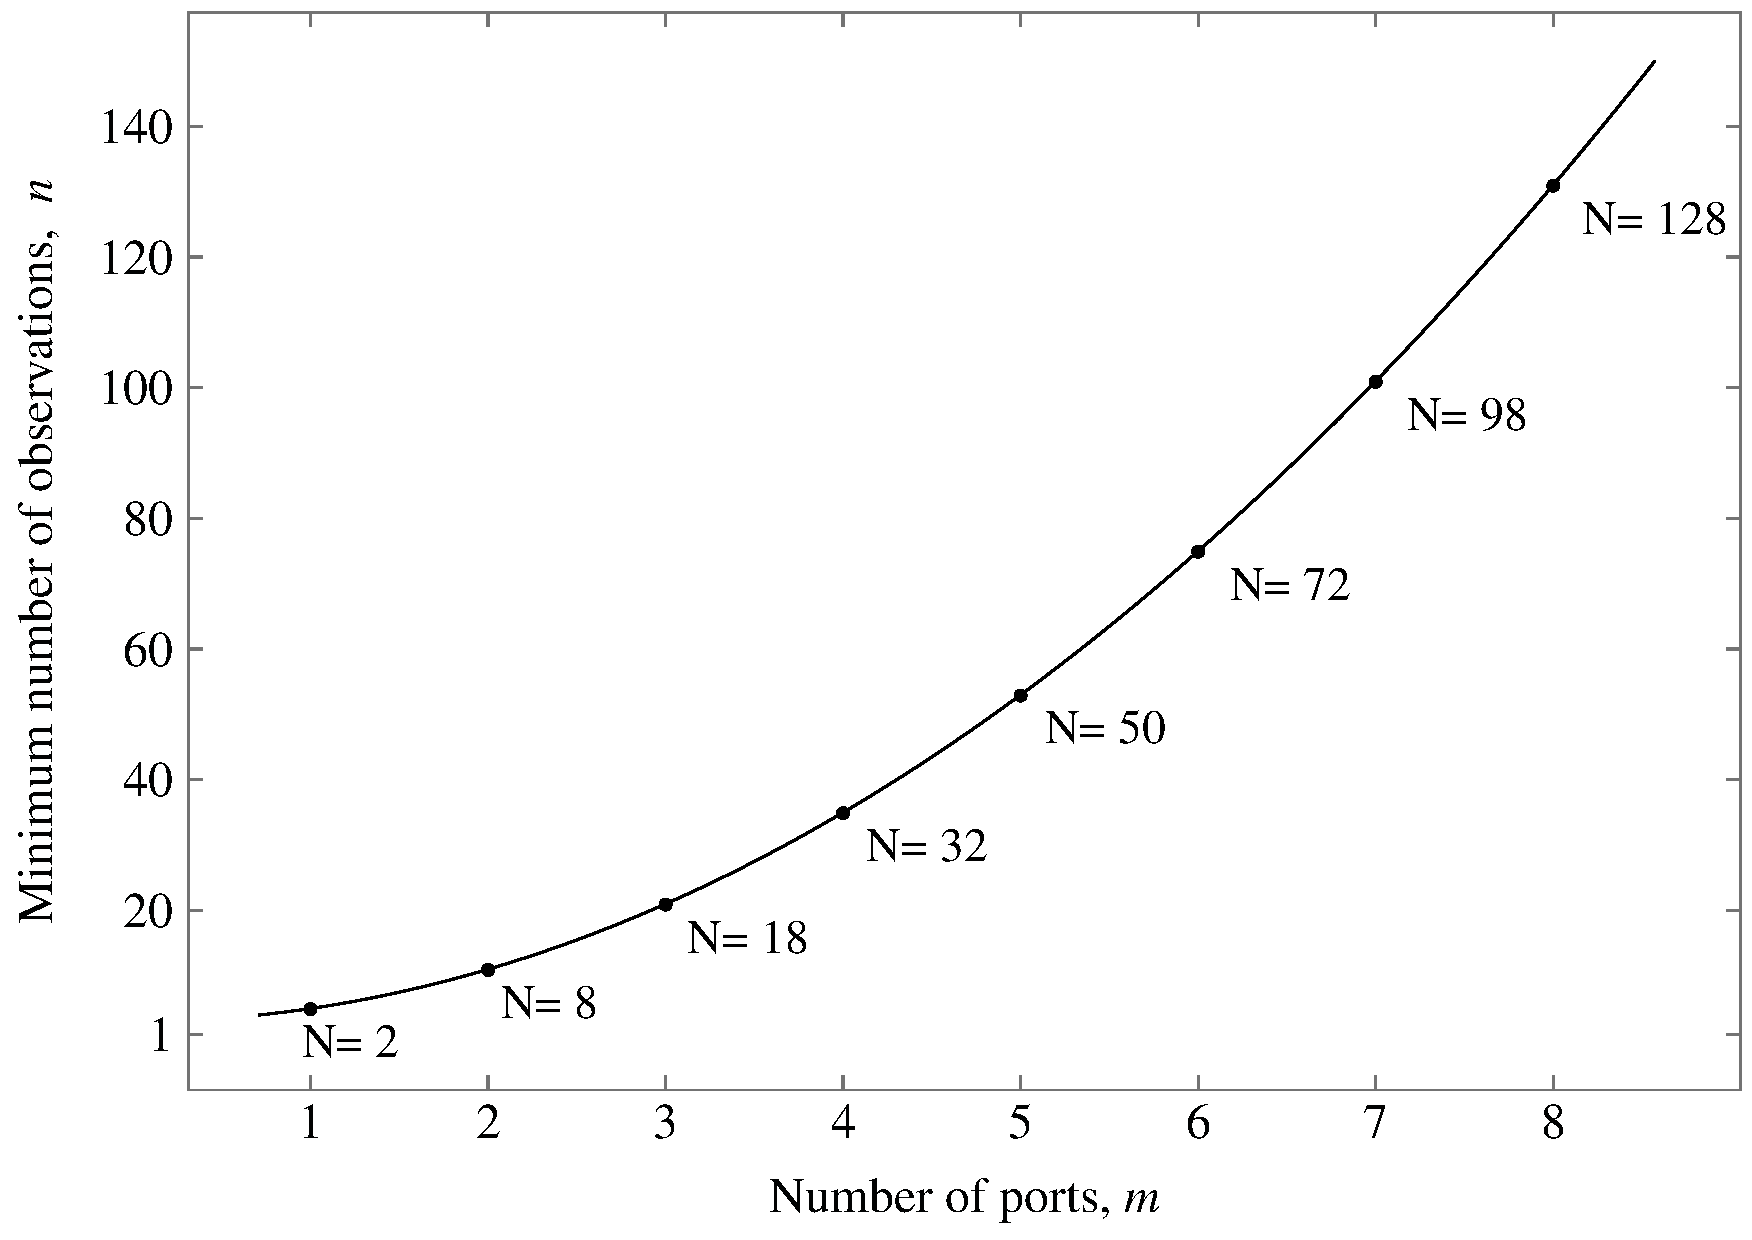
\includegraphics[width=0.8\textwidth]{gum_sparams.pdf}
	\caption[Plot of minimum observations for valid GUM Supplement uncertainty evaluation.]{The minimum number of observations, $n$, required to calculate the standard uncertainty of a full set of S-parameters for a microwave device with m ports using the GUM-S2 approach. The number of input quantities, $N$, for each device is also shown.}
	\label{ch3_fig_gum_sparams}
\end{figure}

\paragraph{Discussion}

The inconsistency of the approaches used in the GUM and its supplements to calculate the standard uncertainty of Category A input quantities of a measurement has two noticeable consequences:

\begin{enumerate}
	\item There can be a large difference in the standard uncertainties reported by each approach. It is not straightforward to decide which is the correct approach to use, however the GUM approach is likely to be more attractive to commercial laboratories and test engineers since this leads to achieving smaller uncertainties in their results.
	\item For situations involving multiple Category A input quantities, the Bayesian approach introduced in the GUM-S1/S2 can require a large number of observations before the standard uncertainty can be defined. Although the standard uncertainty calculated using the GUM approach will become less reliable with fewer observations, it is still possible to obtain a result with only two observations of any number of input quantities. In a commercial laboratory the additional measurements required by the GUM-S1/S2 approach can be impractical, with many laboratories typically using only two or three measurements per device following the GUM approach. For a single input quantity this would require a potential doubling of the number of observations and therefore the test duration, which would either slow throughput or require more test stations to be added. If implemented, the additional time or financial investment would then produce uncertainties that are significantly larger than those obtained using the GUM approach.
\end{enumerate}

This inconsistency is yet to be resolved, and the draft of an updated GUM which replaced much of the remaining classical approach with Bayesian techniques received many poor reviews when circulated for discussion. Work is now being carried out to find solutions to the issues raised by converting to a fully Bayesian GUM. Specific to the example presented in this Section, an article was recently published which offers a way to use Bayesian statistics to evaluate uncertainty in Category A input quantities with $n \ge 2$ repeat observations, which is the same number required by the classical approach \cite{Cox_2017}.

For the work in this thesis, which is based on multivariate electromagnetic measurement problems, the GUM approach (instead of the Supplement 2 approach) is used. In addition, an existing software framework, introduced later, which is included as part of the complete framework presented in this work, also uses the GUM approach for processing Category A uncertainty components.

\subsubsection{Category B Evaluation}

Category B uncertainty components are those which have not been obtained by repeated measurements. Possible sources include previous measurement data, experience or knowledge of relevant materials and instruments, manufacturer’s specifications, data provided by calibration and other certificates and reference data from handbooks.

Values obtained from these sources will typically be an estimate accompanied by either a standard uncertainty or an expanded uncertainty. The latter can be converted to a standard uncertainty, the process of which is described in Section 3.6. Category B uncertainty components are not restricted to Gaussian or t-distributions, and could for example be normal (rectangular), beta, or Cauchy distributions. Unless the combined standard uncertainty is determined via a Monte Carlo method, as explained in the following section, the standard uncertainty must be known for the value to be used as an input quantity.

\subsection{Evaluating Combined Standard Uncertainty}

In order to determine the standard uncertainty of the measurand (the combined standard uncertainty) the uncertainties of the input quantities must be propagated through the measurement model. The GUM offers several methods to achieve this, which will be described in this section.

\subsubsection{Monte Carlo Methods}

Supplement 1 of the GUM \cite{GUM_S1} covers the use of a Monte Carlo technique to determine combined standard uncertainty in the measurand. The Monte Carlo technique has three important benefits for the propagation of uncertainty:

\begin{enumerate}
	\item The measurement model does not need to be known explicitly. In some cases, the algorithm used to obtain a measurement result is proprietary and cannot be made available to the metrologist. Alternatively, the measurement model may be very complicated or involve numerical solutions which cannot be differentiated as required by other propagation methods.
	\item Full knowledge of the probability distributions of the input quantities are used and preserved through the uncertainty propagation. Because the input quantity distributions are sampled directly, the complete probability distribution of the measurand can be obtained (see Figure \ref{ch3_fig_distributions}). This can be very useful when more exotic distributions such as u-shaped distributions are used for input quantities, or if the measurement model is strongly nonlinear, when one cannot make assumptions about the probability distribution of the measurand.
	\item The uncertainty propagation preserves nonlinearities in the measurement model. Alternative propagation methods presented in the GUM cause the measurement model to be linearised around the estimate. In most cases where a nonlinear measurement model is used, however, the uncertainty values are sufficiently small that a linear approximation is valid \cite[5.1.5]{GUM_2008}. Often, an initial Monte Carlo propagation is used to validate this assumption.
	\item All correlations between input quantities are preserved. For many measurements involving multiple input quantities (especially in electromagnetic measurements), the uncertainties of one or more input quantities may be correlated. This means that when the value of one quantity changes, it affects the values of others. This can both increase or decrease the combined standard uncertainty in the measurand significantly. Chapter 4 will discuss the impact of correlations on VNA measurements.
\end{enumerate}

\begin{figure}
	\centering
	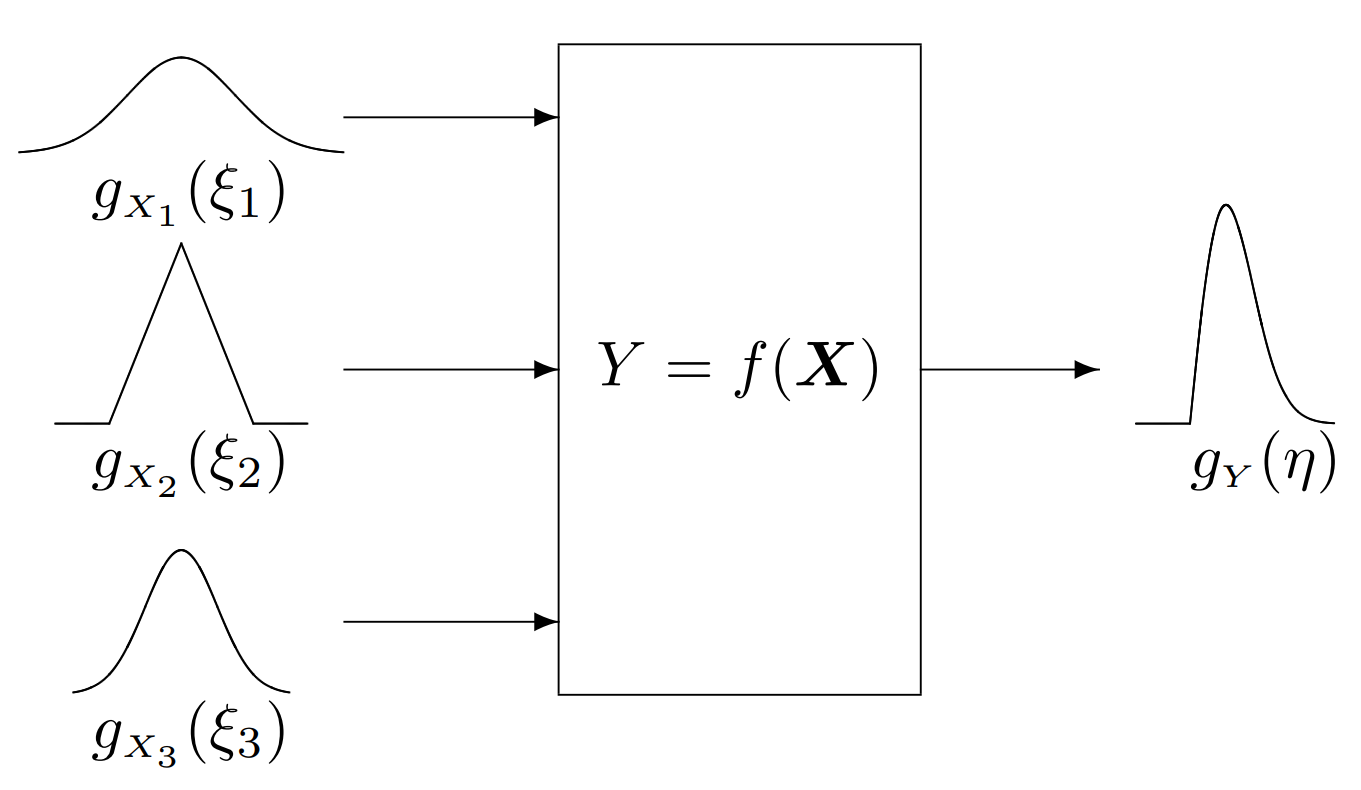
\includegraphics[width=0.65\textwidth]{distributions}
	\caption[Propagation of probability distributions used in GUM Supplement 1.]{An illustration of the propagation of distributions from three input quantities $g_{X1}$, $g_{X2}$, $g_{X3}$, through the measurement model, $Y$, to the measurand, $g_{Y}$ \cite{GUM_S1}.}
	\label{ch3_fig_distributions}
\end{figure}

The primary disadvantage of Monte Carlo methods is the time required to process them. For an accurate evaluation of uncertainty, the number of samples must be sufficiently large. Generally, the GUM recommends 106 samples for a 95\% coverage interval accurate to one or two significant digits \cite[7.2.1]{GUM_S1}. The number of samples increases with the size of the desired coverage interval of similar accuracy. For many measurements today, the processing power of modern computers is sufficient for the duration of uncertainty propagations using Monte Carlo methods to be acceptable. However, in situations where the measurement model is very time-consuming to process, or where the uncertainty evaluation must be very fast, linear propagation techniques may be preferred. A detailed explanation of the steps involved in performing a Monte Carlo propagation can be found in Section 7 of \cite{GUM_S1}.

\subsubsection{Law of Propagation of Uncertainty}

The primary propagation method presented in the GUM is the Law of Propagation of Uncertainty (LPU). This method uses first-order derivatives of the measurement model, together with the variances (and co-variances) of the input quantities, to determine a value for the combined standard uncertainty. The use of first-order derivatives means that the measurement model is linearised, which in many applications can be a valid assumption. The LPU provides different equations for combining independent (uncorrelated) and correlated input quantities. For independent input quantities,

\begin{equation}
u^2_c(\bar{y}) = \sum_{i=1}^{N}(\frac{\partial f}{\partial x_i})^2 u^2(\bar{x}_i),
\end{equation}

where $u^2_c(\bar{y})$, the combined variance, is the square of the combined standard uncertainty, $f$ is the function describing the measurement model, and $x_i$ is an input quantity with variance $u^2(\bar{x}_i)$. For correlated input quantities (whose covariances always form a symmetric and positive semi-definite matrix),

\begin{equation}
u^2_c(\bar{y}) = \sum_{i=1}^{N}\sum_{j=1}^{N} \frac{\partial f}{\partial x_i}\frac{\partial f}{\partial x_j} u(\bar{x}_i,\bar{x}_j) = \sum_{i=1}^{N}(\frac{\partial f}{\partial x_i})^2 u^2(\bar{x}_i) + 2\sum_{i=1}^{N-1}\sum_{j=i+1}^{N} \frac{\partial f}{\partial x_i}\frac{\partial f}{\partial x_j} u(\bar{x}_i,\bar{x}_j).
\label{ch3_eqn_lpu_corr}
\end{equation}

Supplement 2 to the GUM offers a matrix formulation of (\ref{ch3_eqn_lpu_corr}) \cite[6.2.1.3]{GUM_S2}, which handles the multivariate case where multiple measurands are encountered. If the covariance matrix of dimension $N \times N$ associated with $\bar{\bm{x}}$ is

\begin{align}
\boldsymbol U(\bar{\boldsymbol x}) & = 
\begin{bmatrix}
u{(\bar{\boldsymbol x}_1,\bar{\boldsymbol x}_1)}&\dots&u(\bar{\boldsymbol x}_1,\bar{\boldsymbol x}_n)\\
\vdots&\ddots&\vdots\\
u(\bar{\boldsymbol x}_n\bar{\boldsymbol x}_1)&\dots&u{(\bar{\boldsymbol x}_n,\bar{\boldsymbol x}_n)}
\end{bmatrix}
\end{align}

the covariance matrix of dimension $m \times m$ associated with $\bar y$ is

\begin{align}
\boldsymbol U(\bar{\boldsymbol y}) & = 
\begin{bmatrix}
u{(\bar{\boldsymbol y}_1,\bar{\boldsymbol y}_1)}&\dots&u(\bar{\boldsymbol y}_1,\bar{\boldsymbol y}_n)\\
\vdots&\ddots&\vdots\\
u(\bar{\boldsymbol y}_n\bar{\boldsymbol y}_1)&\dots&u{(\bar{\boldsymbol y}_n,\bar{\boldsymbol y}_n)}
\end{bmatrix}
\end{align}

and the sensitivity matrix $\boldsymbol C_{\bar{\boldsymbol x}}$ of dimension $m \times N$ containing the first-order partial derivatives of the measurement model to each input quantity (the Jacobian of the measurement model) is given by evaluating

\begin{align}
\boldsymbol C_{\bar{\boldsymbol x}} & = 
\begin{bmatrix}
\displaystyle \frac{\partial f_1}{\partial X_1}&\dots&\displaystyle \frac{\partial f_1}{\partial X_N}\\
\vdots&\ddots&\vdots\\
\displaystyle \frac{\partial f_m}{\partial X_1}&\dots&\displaystyle \frac{\partial f_m}{\partial X_N}
\end{bmatrix}
\label{ch3_eqn_sens_matrix}
\end{align}

at $\boldsymbol X = \bar{\boldsymbol x}$, then $\boldsymbol U_{\bar{\boldsymbol y}}$ is given by

\begin{equation}
\boldsymbol U_{\bar{\boldsymbol y}} = \boldsymbol C_{\bar{\boldsymbol x}}\boldsymbol U_{\bar{\boldsymbol x}}\boldsymbol C_{\bar{\boldsymbol x}}^\top
\end{equation}

The LPU does not provide any information about the shape of the probability distribution of $\boldsymbol U_{\bar{\boldsymbol y}}$ or its components. The results of the measurement are obtained from the estimates and the combined standard uncertainties – the positive square roots of the diagonal terms of the covariance matrix.

\subsubsection{Finite Difference Methods} \label{ch3_sec_fd_methods}

Included in the definition of the LPU is an alternative method of determining the sensitivity coefficients in (\ref{ch3_eqn_sens_matrix}), without the need to know the measurement model, $f$, explicitly. This technique can be described as a finite difference method and involves measuring the change in $Y$ while varying a particular $X_i$ and holding all other input quantities constant. This is often used when there may not be a model available for a particular process but a rudimentary uncertainty analysis is required, or if the computational power is available to recompute the finite differences when the estimates change. Typically, the sum of the estimate and the standard uncertainty of each input quantity $\bar{x}_i + u(\bar{x}_i)$ is used, although a more rigorous version also includes the standard uncertainty subtracted from the estimate $\bar{x}_i + u(\bar{x}_i)$ to check for asymmetry. Because only two points are used to solve for each sensitivity coefficient (the estimate and the estimate plus standard uncertainty), this uncertainty propagation also linearises the measurement model.

If all of the input quantities are considered independent and the standard uncertainty was chosen as the value with which to perturb the input quantities, then by subtracting the estimate of the measurand from each sample and adding the results in quadrature, the combined standard uncertainty in the measurand can be obtained:

\begin{equation}
u_c(\bar{y}) = \sqrt{\sum_{i=1}^{N}((\bar{x}_i+u(\bar{x}_i))-\bar{x}_i)}
\end{equation}

\subsection{Expanded Uncertainty and Coverage Intervals}

Although it is recommended to express a result with combined standard uncertainty $u_c({\bar{y}})$, it is often required, especially in safety critical applications, for the uncertainty to encompass a larger fraction of the distribution of values that could reasonably be attributed to the measurand. An expanded uncertainty, $U$, is instead used and is related to the combined uncertainty by $U=ku_c(\bar{y})$ \cite[6.2.1]{GUM_2008}. The multiplying factor, $k$, is termed the coverage factor and is typically in the range 2 to 3, often either of those two integer values and is defined by specifications or standards relating to the application.  Using expanded uncertainties, the result can be expressed as $\bar{y} \pm U$, which is a popular format for datasheets and specifications.

To obtain a coverage factor that states a probability (e.g. 95\%) that the true value of a measurand is within the associated interval is not straightforward, and depends on the probability distribution of the measurand. If all input quantities are Category A uncertainty components and the measurement model is linear, then the measurand distribution can be assumed to be Gaussian. In this case, the coverage interval is known as a confidence interval and can be given as a percentage by  $\erf(z/\sqrt{2})\times 100$, where $\erf(x)$ is the Gauss error function of $x$.
 
In situations where the above conditions cannot be met, a level of confidence can be obtained by calculating the effective degrees of freedom $\nu_\text{eff}$ of the distribution of the measurand. This process is explained in Annex G of [5]. For Monte Carlo propagations with sufficient samples, the confidence interval can be found by analysing the distribution of the measurand and obtaining the deviation from the estimated value which encompasses the desired percentage of samples (e.g. 95\%).

\section{Sensitivity Analysis}

A benefit of propagating uncertainties through the measurement model is that an analysis of the sensitivity of the measurands to each input quantity can be performed. The sensitivity coefficients obtained from the measurement model can either be compared directly or multiplied by the standard uncertainty of the respective input quantity, in order to obtain an uncertainty figure for the measurand which can be compared with those calculated for other input quantities. This method is similar to the finite difference propagation technique described in \ref{ch3_sec_fd_methods}, which can also be used to perform a sensitivity analysis. Because the input quantities are perturbed from their estimate sequentially (while all others are held at their estimate), this form of sensitivity analysis is termed ``sequential perturbation''.

The results of the sensitivity analysis can be very useful to the metrologist. Not only can the relative impact of different input quantity uncertainties be reviewed, but also complicated behaviour in the combined standard uncertainty may be better understood; Figure \ref{ch3_fig_sensitivity} shows an example. Sensitivity analyses are also an efficient approach to reducing combined standard uncertainty. Once input quantities with dominant contributions have been identified they can be targeted for improvement – or in some cases an alternative measurement model can be used which avoids them.

\begin{figure}[h!]
	\centering
	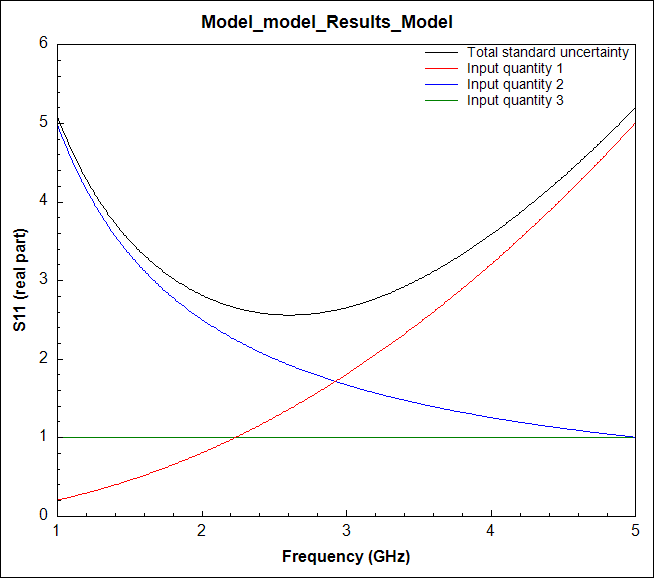
\includegraphics[width=0.8\textwidth]{sensitivity}
	\caption[Sensitivity analysis example results.]{An example of results from a sensitivity analysis which reveal the origins of the complicated behaviour of the combined standard uncertainty with respect to a variable (in this case frequency).}
	\label{ch3_fig_sensitivity}
\end{figure}

\section{Conclusions}

This chapter presented how measurements underpin modern life, supporting trade and commerce and facilitating new discoveries in science and engineering. Through traceability and the unit system, the evaluation and management of uncertainty in measurements generates confidence and trust. In an attempt to standardise the definition and representation of measurement uncertainties, an internationally-used guidance document, the GUM, offers rigorous methods to evaluate these uncertainties. However, the GUM continues to be developed, and recently an inconsistency was created in the evaluation of Category A uncertainty components. This chapter has reviewed the inconsistency from the objective of electromagnetic measurements, an area of metrology where the effects have been shown to be potentially significant.

Three methods for propagating uncertainty through a measurement model to determine the combined standard uncertainty of the measurands were described. Although the Monte Carlo method preserves the most information about both the uncertainties of the input quantities and the measurement model, the higher computational effort can be prohibitive in some cases. Instead, the LPU provides two linear alternatives, which are often much more efficient but require validation to ensure that the measurement model can be treated as linear.

The idea of expanded uncertainty and coverage intervals was introduced, these being met frequently in Category B uncertainty components defined from datasheets and specifications. A confidence interval is straightforward to calculate if the measurement involves only Category A uncertainty components and has a linear measurement model, or if a Monte Carlo propagation is used and the probability distribution of the measurand can be attributed to a standard type. In other cases, a coverage interval can be calculated using knowledge of the input quantities and further guidance from the GUM.

Finally, this chapter described sensitivity analysis, which can be carried out using results from the LPU procedure. The framework presented in this thesis utilises a sensitivity analysis to allow the user to examine and attempt to minimise significant sources of uncertainty, which is especially important in sensitive electromagnetic measurements such as those made on-wafer.

%\addcontentsline{toc}{section}{Bibliography}
%\printbibliography[title=References]
%\end{refsection}
\end{document}
